\chapter[PROJETO E IMPLEMENTAÇÃO DO SERVIÇO DE PROCESSAMENTO]{PROJETO E IMPLEMENTAÇÃO DO SERVIÇO DE PROCESSAMENTO}

\label{chapter:architecture}

Escolhemos a \textbf{Arquitetura Kappa} como padrão de projeto para servir
de base para o novo serviço de processamento de dados do InterSCity.
A Arquitetura Lambda não justifica a maior complexidade no contexto atual da
plataforma, de modo que essa escolha facilita a manutenibilidade e adoção do
serviço pelo time atual do InterSCity. A Arquitetura Kappa permitirá a análise
em tempo-real sem que ocorra perda de informações relevantes, o que é
importante no contexto de cidades inteligentes, ao passo em que permite a
análise de dados históricos, desde que tenha ocorrido o pré-processamento.
Essa decisão resultou na necessidade de escolha de uma tecnologia de
processamento de fluxos e de um \textit{broker} adequado.

\begin{figure}[hbt]
  \centering
    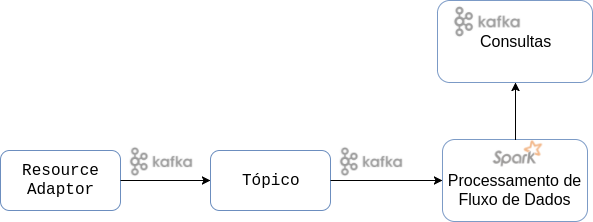
\includegraphics[scale=0.5]{figuras/kappa_tools2.png}
  \caption{Pilha de tecnologias utilizadas - Apache Kafka e Apache Spark, e suas
    interações com o InterSCity.}
  \label{fig:stack}
\end{figure}

Escolhemos o \textbf{Apache Spark} como tecnologia de processamento de fluxos
a ser usada, por dispor nativamente de biblioteca de clusterização
e aprendizagem de máquina. O Spark ainda facilita, caso necessário, a
troca para a Arquitetura Lambda, por dispor de processamento \textit{batch}.
Escolhemos o \textbf{Apache Kafka} como o \textit{broker} do novo serviço de
processamento, sendo essa uma escolha menos óbvia que a anterior. Embora o
RabbitMQ já seja utilizado pelo InterSCity e tenha vantagens em certos aspectos
em relação ao Kafka, tomamos essa decisão pelo RabbitMQ não dispor de uma
interface nativa que o conecte ao Spark. Outro fator que levamos em conta é o
fato do Kafka ter gerenciamento nativo de \textit{log}, que ajuda na
implantação da Arquitetura Kappa. Contudo, só utilizamos o Kafka no serviço
de processamento de dados, não forçando mudanças no ecossistema de
microsserviços do InterSCity. A Figura \ref{fig:stack} ilustra a pilha de
tecnologias que deve compor a Arquitetura Kappa no InterSCity e as principais
relações entre os diferentes serviços.

\section{IMPLEMENTAÇÃO}

Dividimos a implementação da Arquitetura Kappa em três etapas:
(1) configuração do ambiente, contemplando as ferramentas escolhidas;
(2) ligações entre os diferentes serviços, tornando possível a publicação de
    mensagens no Kafka e sendo possível seu processamento no Spark; e
(3) disponibilização de \textit{hooks} que possam ser estendidos futuramente,
    possibilitando a criação de um canal de dados customizável.

Durante a implementação do novo serviço de processamento de dados para o
InterSCity desenvolvemos o \textbf{Shock}, responsável por abstrair as
comunicações entre as diferentes ferramentas e trazer a extensibilidade mencionada
na terceira etapa da implementação. O Shock é uma aplicação que compõe o
novo serviço de processamento, junto com outras aplicações utilizadas, e
possibilita que usuários que não conhecem o Apache Spark consigam requisitar
processamento e análise de fluxos de dados.

\begin{figure}[hbt]
  \centering
    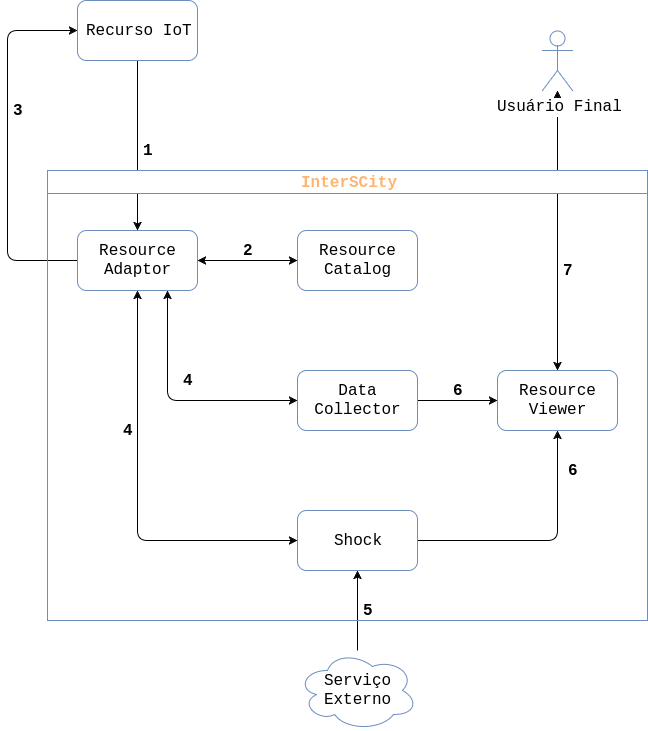
\includegraphics[scale=0.45]{figuras/shock_usage.png}
    \caption{Novo ciclo de vida da plataforma, com relação ao novo serviço de processamento.}
  \label{fig:shock_usage}
\end{figure}

A Figura \ref{fig:shock_usage} ilustra o novo fluxo completo do InterSCity com a
adição do novo serviço de processamento de dados. O início do fluxo (passos 1 ao
3) continua o mesmo, e começa com (1) um recurso IoT se registrando na plataforma
através da interação com o Resource Adaptor. O Resource Adaptor (2) cadastra o
recurso no microsserviço Resource Catalog (3) e informa o UUID que deve ser
utilizado pelo recurso. O recurso passa a enviar dados ao Resource Adaptor, que
(4) publica a chegada dos novos dados no Shock através do Kafka, promovendo
extensão ao InterSCity.  Aplicações (5) interagem com o Shock via Kafka,
construindo o canal de um fluxo de dados, definindo as operações a
serem executadas.  Por fim, os resultados do Shock e do Data Collector (6)
serão disponibilizados, podendo ser consumidos por aplicações como o
microsserviço Resource Viewer, que (7) apresenta dados ao usuário final.

Assim como seguido pela equipe do InterSCity, utilizamos o Docker na gerência de
configuração do novo serviço. A configuração do Spark que havia sido feita pelo
time do InterSCity na criação do DataProcessor foi reutilizada, e configuramos
um contêiner com o Kafka. Por fim, ligamos os contêineres configurados com o
microsserviço Resource Adaptor, permitindo assim a interação entre o InterSCity
e as ferramentas definidas para uso.

Iniciamos a ligação entre os projetos, etapa 1, com uma adaptação no
microsserviço Resource Adaptor, que com a mudança, passou a publicar em um tópico
específico no Kafka a chegada de novos dados. Essa adaptação não trouxe mudanças
significativas no InterSCity, não afetando o fluxo usual da plataforma.
Após, solucionamos as etapas 2 e 3 através do desenvolvimento do Shock,
responsável por receber mensagens em tópicos específicos do Kafka e passá-los
ao Spark Streaming. O Shock gerencia a execução de fluxo de dados do Spark,
permitindo que usuários terceiros configurem fluxos de dados no Spark sem ter
conhecimento técnico da ferramenta.

\section{SHOCK}

O Shock encontra-se disponível em um repositório no
Gitlab\footnote{\url{https://gitlab.com/DGuedes/shock}}, e o novo microsserviço
de processamento de dados pode ser encontrado em um \textit{fork} do serviço
original\footnote{\url{https://gitlab.com/DGuedes/data-processor}}. O Shock
abstrai o uso das diferentes ferramentas e pode ser customizado
por serviços externos que definem e configuram fluxos para serem
executados. A arquitetura do Shock apresenta pontos de estensão e possui
um \textit{handler} para a Arquitetura Kappa
desenvolvido\footnote{\url{https://gitlab.com/DGuedes/shock/blob/master/shock/handlers.py}},
mas caso seja desejado o uso de outra estratégia, basta implementar um novo
\textit{handler}.

\pagebreak

\begin{figure}[hbt]
  \centering
    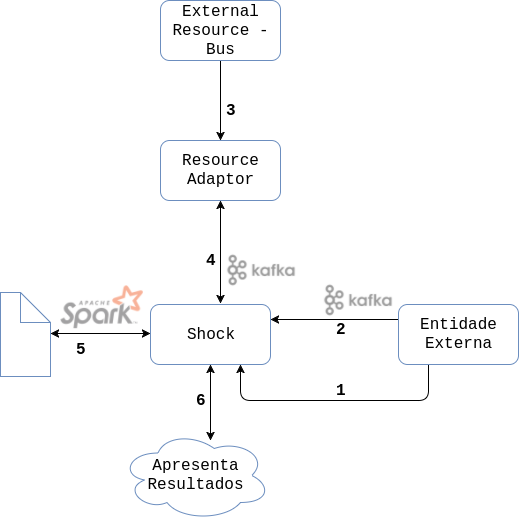
\includegraphics[scale=0.45]{figuras/shock.png}
    \caption{Ciclo de vida do Shock dentro do InterSCity.}
  \label{fig:shock}
\end{figure}

A Figura \ref{fig:shock} ilustra o uso do Shock, utilizando como exemplo uma
aplicação de cidades inteligentes desenvolvida pelo time do
InterSCity\footnote{\url{https://gitlab.com/smart-city-software-platform/external-resources/tree/master/bus}},
que disponibiliza dados como as coordenadas, o tempo, o índice e a linha de
alguns ônibus de São Paulo. Imaginando que seja desejado a criação de uma nova
informação a partir dos dados dos ônibus, como a \textit{velocidade}, o fluxo
de uso com o Shock poderia ser: (1) um cliente que deseje utilizar o serviço
de processamentos do InterSCity analisa as funções que o Shock disponibiliza
para criação do fluxo, e (2) constrói o fluxo desejado através
dessas funções, via Kafka. Os recursos IoT (3) publicam no Resource Adaptor a
chegada de novos dados de ônibus, para que esses dados sejam (4) publicados em
um tópico específico do Kafka pelo Resource Adaptor. Após serem disponibilizados
no Kafka, os dados ficam disponíveis para serem utilizados pelo Shock, que os (5)
recebe nos fluxos de dados configurados para ingerir dados, e os processa
através do canal construído no passo 2. Por fim, após o
processamento dos dados, o Shock pode (6) disponibilizar os resultados do
processamento, que pode ser reaproveitado por aplicações terceiras.

\begin{figure}[hbt]
  \centering
  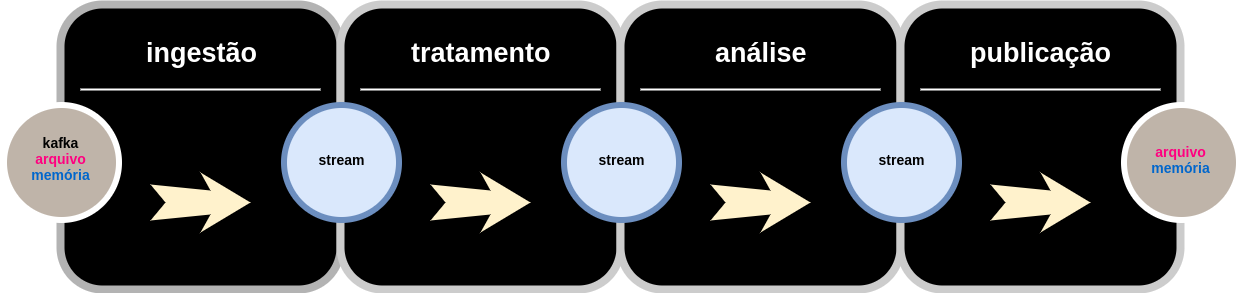
\includegraphics[scale=0.35]{figuras/arquiteturaforensic.png}
  \caption{Padrão \textit{ingest, setup, analyze e publish.}}
  \label{fig:ingeststore}
\end{figure}

Do ponto de vista da implementação, utilizamos no Shock a arquitetura de camadas
\textit{ingestão, tratamento, análise e publicação}, cujas traduções em inglês são
respectivamente \textit{ingest, store, analyze} e \textit{publish}. Essa arquitetura
é apresentada na Figura \ref{fig:ingeststore}, e a criamos para o Shock utilizando
como base arquiteturas mais difundidas, como a \textit{ingest, store, analyze} e
\textit{visualize}, utilizada na plataforma Google Cloud
Platform\footnote{\url{https://cloud.google.com/solutions/data-lifecycle-cloud-platform}},
e a arquitetura \textit{collecton tier, message queuing tier, analysis tier,
in-memory data store} e \textit{data access tier}, explicada por
\citeonline{psaltis2017streaming}. No Shock, cada uma dessas camadas são
classificadas como estágios de um fluxo de dados, podendo um
fluxo de dados ter no máximo 4 estágios.

Diferente dos outros serviços da plataforma, as aplicações clientes podem interagir
com o Shock através de uma API fornecida via o Kafka. Assim, as aplicações enviam
mensagens ao Kafka utilizando um formato semelhante ao JSON, com o padrão ``arg1;\{arg2\}'',
onde o primeiro \textit{token}, ``arg1'', representa o nome
da ação desejada, e o segundo, ``arg2'', os argumentos da ação. Um
\textit{handler} no Shock receberá a ação requisitada no método
\textit{handle}, e deve tratar a requisição recebida. Por exemplo, uma mensagem
\small{\textbf{ingestion;\{"stream": "mystream", "shock\_action": "socketIngestion"\}}},
deve ser enviada caso queira-se o registro de um estágio de ingestão no
fluxo de dados \textit{mystream} utilizando a estratégia \textit{socketIngestion}.

\begin{figure}[hbt]
  \centering
    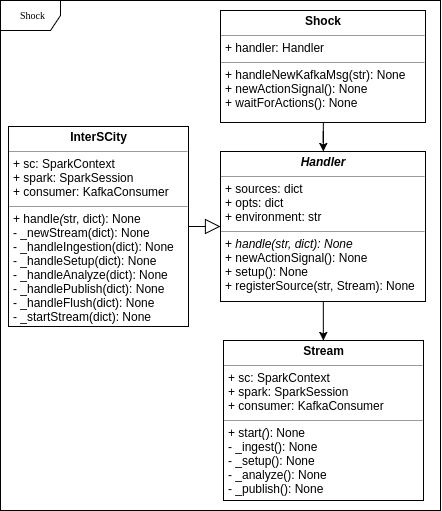
\includegraphics[scale=0.5]{figuras/ShockUML.png}
  \caption{Diagrama de classes do Shock.}
  \label{fig:uml}
\end{figure}

A Figura \ref{fig:uml} apresenta o diagrama das principais classes do Shock. O
núcleo do Shock é representado pela classe Shock, que sustenta-se no uso de um
\textit{handler} que implemente o método \textit{handle}. Atualmente, um
\textit{handler} para o InterSCity encontra-se implementado, contudo, caso
seja desejado o uso de um \textit{handler} que utilize a Arquitetura Lambda, por
exemplo, basta a criação de uma nova classe que herde da classe
\textit{Handler} e que implemente o método \textit{handle} para as diferentes
ações requisitadas. Por fim, uma classe \textit{Stream} utiliza a arquitetura
de camadas citada anteriormente, onde cabe ao \textit{handler} gerenciar e
interagir com os diferentes fluxos de dados criados.

\lstinputlisting[label={lst:ingestion},caption={
  Ingestão de dados no Shock via \textit{socket} e Kafka.
  }]{editaveis/arquivos/ingestion.py}

O primeiro estágio de um fluxo de dados, a \textit{\textbf{ingestão}}, trata-se da
ingestão dos dados a partir de alguma fonte, como algum tópico do Kafka, ou
algum arquivo novo. Atualmente o Shock fornece três tipos diferentes de
ingestão: ingestão via tópico do Kafka, ingestão via arquivo (Parquet e JSON)
e ingestão via \textit{socket}. A depender da estratégia de ingestão, alguns
parâmetros são necessários na configuração - numa ingestão via Kafka, por
exemplo, é necessário configurar o endereço do \textit{broker} e os tópicos
que serão utilizados. A Listagem \ref{lst:ingestion} apresenta o código-fonte
de duas estratégias de ingestão disponíveis no Shock.

\lstinputlisting[label={lst:setup},caption={
  Tratamento de dados no Shock via \textit{cast}.
}]{editaveis/arquivos/store.py}

O segundo estágio de um fluxo de dados é chamado \textit{\textbf{preparo}} e tem o papel
de ajuste e limpeza dos dados para que sejam utilizados pelos fluxos
sem maiores complicações. Um exemplo típico é o uso de um estágio de preparo
que faça \textit{cast} (mudanças nos tipos de dados) de dados, quando valores estão como
\textit{string} quando são necessários valores \textit{double}. Atualmente,
o Shock apresenta somente preparo de dados via \textit{cast}, que são essenciais
no uso do InterSCity e de consumo do Kafka, apresentados na Listagem
\ref{lst:setup}.

\lstinputlisting[label={lst:analyze},caption={
  Operações de análise de dados no Shock.
}]{editaveis/arquivos/processing.py}

O terceiro estágio de um fluxo, a \textit{\textbf{análise}}, é o
estágio principal do processamento, e permite filtros, agregações e cálculos.
No Shock, a etapa de análise dos dados recebe como entrada um um fluxo de dados
de dados e retorna um fluxo de dados transformado. Uma aplicação que deseje
utilizar a operação de filtro no fluxo \textit{mystream} com a finalidade
de filtrar os valores de \textit{air\_quality} iguais a 31, deve fazer uma
requisição no Kafka com o conteúdo \small{\textbf{processing;\{"stream": "mystream",
"shock\_action": "streamFilter", "query": "select * from air\_quality where
'value' == 31"\}}}. Algumas possibilidades de estágios de análise
estão contidos na Listagem \ref{lst:analyze}.

\lstinputlisting[label={lst:publish},caption={
  Estratégias de publicação de resultados presentes no Shock.
}]{editaveis/arquivos/sinks.py}

O último estágio de um fluxo de dados, conhecido como estágio de
\textit{\textbf{publicação}}, é o estágio
de apuração do processamento, retornando os dados necessários para o cliente.
O Shock atualmente permite a publicação via arquivo, memória e \textit{console}, e após o
lançamento da versão 2.2 do Spark, permitirá a publicação via Kafka. A
publicação via arquivo é limitada, pois não permite a publicação em um servidor
externo. A publicação via memória também não permite, mas é interessante pois
o conteúdo passa a estar disponível para ser requisitado via SparkSession,
permitindo consultas com sintaxe SQL. Por fim, a publicação via \textit{console} está
presente somente para fins de desenvolvimento, mas é possível que ocorra uma
combinação com outras ferramentas que leiam da saída padrão do Sistema Operacional.
Categorizamos no Shock o nome \textit{sink} para as diferentes estratégias de
publicação, que é o nome utilizado pelo Spark. A Listagem \ref{lst:publish}
apresenta as estratégias de publicação em \textit{console}, Parquet e memória.

\begin{figure}[hbt]
  \centering
    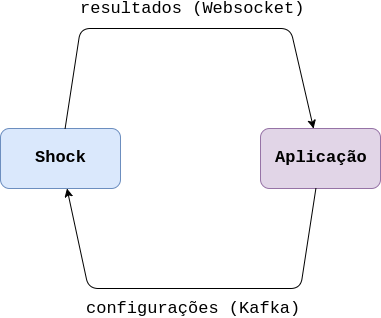
\includegraphics[scale=0.5]{figuras/ligacoes.png}
  \caption{Comunicação entre o Shock e aplicações.}
  \label{fig:ligacoes}
\end{figure}

Como alternativa às limitações de publicação dos dados, o Shock
disponibiliza na API os \textit{flushes}, que atuam como \textit{jobs} adicionais
que ingerem dados de alguma fonte (que não seja um fluxo) e publicam
em outra. Essa alternativa não precisaria existir caso a publicação via Kafka
já estivesse disponível no Spark, mas enquanto o lançamento da versão 2.2 não
ocorre, acaba sendo uma opção válida. Nesse sentido, uma aplicação cliente do
InterSCity poderia usar o Shock para realizar processamento de seus dados
seguindo o fluxo de interação da Figura \ref{fig:ligacoes}. Nessa interação, a
aplicação faz definições no Shock via Kafka, e o Shock apresenta os resultados
pelos estágios de publicação ou por WebSocket.
